%!TEX program = xelatex
\documentclass[aspectratio=169]{ctexbeamer}
\usepackage{multicol}
\usepackage{amsfonts,amsmath,amscd,amssymb,amsthm}
\usepackage{latexsym,bm}
\usepackage{cite}
\usepackage{mathtools,mathdots,graphicx,array,mathrsfs}
\usepackage{fancyhdr}
\usepackage{lastpage}
\usepackage{color}
\usepackage{enumitem}
\usepackage{diagbox}
\usepackage{xcolor,tcolorbox,tikz,tkz-tab,mdframed,tikz-cd}
\usepackage{framed}
\usepackage{verbatim}
\usepackage{extarrows}
\usepackage{fontspec}
\usepackage{hyperref}
\usepackage{braket}
\usepackage{booktabs}

% \usepackage{physics}  
                        %%% 宽高比说明 %%%%
%% ctexbeamer宏包支持各种宽高比,但本模板只适配了4:3(默认)和16:9的宽高比背景。
%% 添加选项aspectratio=169或aspectratio=43可以更改宽高比,默认是4:3
\usepackage[bluetheme]{ustcbeamer}
% !TeX root = ./main.tex

% 自适应16:9的宽高比设置
\makeatletter
\@ifclasswith{ctexbeamer}{aspectratio=169}{
		\def\backxscale{4/3}\def\backyscale{1}\def\ustcshift{30}
	}{
		\def\backxscale{1.068}\def\backyscale{1.068}\def\ustcshift{0}
	}
\makeatother

\newcommand{\maketitleframe}{
	%取消footline,sidebar
	\setbeamertemplate{footline}[footlineoff]
	%%设置本命令以后的背景如下
	\usebackgroundtemplate{%
			% !TeX root = ./main.tex
\begin{tikzpicture}[y=1pt, x=1pt, yscale=0.474*\backyscale, xscale=0.474*\backxscale, inner sep=0pt, outer sep=0pt]
    % \begin{scope}[cm={{1,0.0,0.0,-1,(0,0)}}]
      \path[fill=themecolor1,even odd rule] (720.4059,0.3515) -- (720.4059,71.1507) --
        (0.3436,71.1507) -- (0.3436,0.3515) -- cycle;
    
    
    
      \path[fill=themecolor2,even odd rule] (0.3436,76.0927) -- (720.4059,76.0927) --
        (720.4059,79.3043) -- (0.3436,79.3043) -- cycle;
    
    
    
      \path[left color=themecolor!80, right color=themecolor,even odd rule] (720.4059,392.4714) -- (0.3436,392.4714) --
        (0.3436,112.2780) -- (720.4059,112.2780) -- cycle;
    
    
    
          \path[even odd rule] (720.4059,392.4714) -- (0.3436,392.4714) --
            (0.3436,112.2780) -- (720.4059,112.2780) -- cycle;
    
    
    
      \path[fill=themecolor1,even odd rule] (0.3436,540.3980) -- (720.4059,540.3980) --
        (720.4059,433.5987) -- (0.3436,433.5987) -- cycle;
    
    
    
      \path[fill=themecolor,even odd rule] (84.0129,392.4714) -- (64.1007,392.4714) ..
        controls (139.6636,296.8146) and (237.7485,213.1007) .. (369.3679,152.9909) ..
        controls (258.0055,213.1787) and (160.4523,292.5573) .. (84.0129,392.4714) --
        cycle(0.3436,210.9419) -- (0.3436,112.2780) -- (205.1827,112.2780) .. controls
        (135.2103,142.0132) and (67.0535,175.1304) .. (0.3436,210.9419) --
        cycle(0.3436,318.0849) -- (0.3436,261.2429) .. controls (87.4868,197.7318) and
        (173.6552,147.4217) .. (257.6874,112.2780) -- (329.6364,112.2780) .. controls
        (208.4627,165.2559) and (97.0387,225.2988) .. (0.3436,318.0849) --
        cycle(23.7974,392.4714) -- (0.3436,392.4714) -- (0.3436,375.5798) .. controls
        (103.8628,248.3597) and (243.0859,163.2623) .. (385.7678,112.2780) --
        (411.7601,112.2780) .. controls (266.1313,174.0682) and (125.2848,246.4444) ..
        (23.7974,392.4714);
    
    
    
      \path[fill=themecolor2,even odd rule] (0.3436,428.6568) -- (720.4059,428.6568) --
        (720.4059,425.4452) -- (0.3436,425.4452) -- cycle;

      \node at(185-\ustcshift,488){\textcolor{themecolor}{
\includegraphics[scale=1]{./theme/ustc_logo_side.pdf}}};
    % \end{scope}
\end{tikzpicture}
	}%
	%封面页
	\begin{frame}%
		\maketitle%
	\end{frame}%
	%设置本命令以后的背景如下
	\usebackgroundtemplate{%
			% !TeX root = ./main.tex
\begin{tikzpicture}[y=1pt, x=1pt, yscale=0.474*\backyscale, xscale=0.474*\backxscale, inner sep=0pt, outer sep=0pt]
% \begin{scope}[cm={{1,0.0,0.0,-1,(0,0)}}]
    \path[left color=themecolor!80,right color=themecolor,even odd rule] (720.4059,540.3980) -- (0.3436,540.3980) --
      (0.3436,478.8258) -- (720.4059,478.8258) -- cycle;



        \path[even odd rule] (720.4059,540.3980) -- (0.3436,540.3980) --
          (0.3436,478.8258) -- (720.4059,478.8258) -- cycle;



    \path[fill=themecolor,even odd rule] (84.0129,540.3980) -- (64.1007,540.3980) ..
      controls (139.6636,519.3777) and (237.7485,500.9814) .. (369.3679,487.7725) ..
      controls (258.0055,500.9987) and (160.4523,518.4420) .. (84.0129,540.3980) --
      cycle(0.3436,500.5071) -- (0.3436,478.8258) -- (205.1827,478.8258) .. controls
      (135.2103,485.3599) and (67.0535,492.6376) .. (0.3436,500.5071) --
      cycle(0.3436,524.0517) -- (0.3436,511.5606) .. controls (87.4868,497.6042) and
      (173.6552,486.5485) .. (257.6874,478.8258) -- (329.6364,478.8258) .. controls
      (208.4627,490.4677) and (97.0387,503.6621) .. (0.3436,524.0517) --
      cycle(23.7974,540.3980) -- (0.3436,540.3980) -- (0.3436,536.6860) .. controls
      (103.8628,508.7296) and (243.0859,490.0294) .. (385.7678,478.8258) --
      (411.7601,478.8258) .. controls (266.1313,492.4040) and (125.2848,508.3087) ..
      (23.7974,540.3980);

  \path[fill=themecolor2,even odd rule] (720.4059,475.6141) -- (0.3436,475.6141) --
    (0.3436,478.8258) -- (720.4059,478.8258) -- cycle;



  \path[fill=themecolor,even odd rule] (0.3436,0.3515) -- (720.4059,0.3515) --
    (720.4059,28.5100) -- (0.3436,28.5100) -- cycle;



  \path[fill=themecolor2,even odd rule] (720.4059,28.5100) -- (0.3436,28.5100) --
    (0.3436,31.7217) -- (720.4059,31.7217) -- cycle;

  \node at(580+\ustcshift,509){\textcolor{white}{
\includegraphics[scale=0.8]{./theme/ustc_logo_side.pdf}}};



% \end{scope}

\end{tikzpicture}
	}%
}%
%
                        %%% ustcbeamer说明 %%%%
%% 宏包使用了TikZ代码形式的背景文件(在子文件夹theme中),默认选项"bluetheme",是科大校徽的蓝色;此外ustcbeamer还内置了红色和黑色主题"redtheme","blacktheme"。

                        %%% 自定义你的主题颜色 %%%
%% 一旦使用了下述命令就会覆盖ustcbeamer的内置颜色选项,你可以设置自己喜欢的RGB色值:
% \definecolor{themecolor}{RGB}{0,150,0} % 这是绿色主题
% \definecolor{themecolor}{RGB}{0,150,150} % 青色主题,也蛮好看的

%% 注意小写rgb和大写RGB表示的色值相差255倍,即RGB{255,255,255}=rgb{1,1,1};
% \definecolor{themecolor}{rgb}{0,0.5,0.3} % 深绿色主题

%% 建议自定义的主题颜色选择偏深色
%%%%%%%%%%%%%%%%%%%%%%%%%%%%%%%%%%%%%%%%%%%%%%%%%%%%%%%%%%%%%%%%%%%%%%


\title[Algebraic structure]{
    PointNet++
}
\author[USTC]{}
\institute[USTC]{
中国科学技术大学
}
\date{\today}
\begin{document}
%\section<⟨mode specification⟩>[⟨short section name⟩]{⟨section name⟩}
%小于等于六个标题为恰当的标题

%--------------------
%标题页
%--------------------
\maketitleframe
%--------------------
%目录页
%--------------------
%beamer 101
\begin{frame}%
	\frametitle{大纲}%
   % \begin{multicols}{2} % 目录分栏
	\tableofcontents[hideallsubsections]%仅显示节
	%\tableofcontents % 显示所节和子节
    % \end{multicols}

\end{frame}%
%--------------------
%节目录页
%--------------------
\AtBeginSection[]{
\setbeamertemplate{footline}[footlineoff] % 取消页脚
  \begin{frame}%
     % \begin{multicols}{2} % 目录分栏

    \frametitle{大纲}
	%\tableofcontents[currentsection,subsectionstyle=show/hide/hide]%高亮当前节,不显示子节
    \tableofcontents[currentsection,subsectionstyle=show/show/hide]%show,shaded,hide
    % \end{multicols}

  \end{frame}
\setbeamertemplate{footline}[footlineon]%添加页脚
}
%--------------------
%子节目录页
%--------------------
\AtBeginSubsection[]{
\setbeamertemplate{footline}[footlineoff]%取消页脚
  \begin{frame}%
    \frametitle{大纲}
	%\tableofcontents[currentsection,subsectionstyle=show/hide/hide]%高亮当前节,不显示子节
    \tableofcontents[currentsection,subsectionstyle=show/shaded/hide]%show,shaded,hide
  \end{frame}
\setbeamertemplate{footline}[footlineon]%添加页脚
}
\setlength{\parindent}{2em}

\section{介绍}

\begin{frame}
  \frametitle{介绍}

点云是一种重要的几何数据结构。由于其不规则的格式,大多数研究人员将这些数据转换为规则的3D体素网格或图像集合。然而,这使得数据不必要地庞大,并造成问题。研究人员设计了一种新型的神经网络PointNet,它直接以点云作为输入,考虑了输入点的排列不变性。PointNet提供了一个统一的架构,用于对象分类,物体分割,场景分割。

\begin{figure}
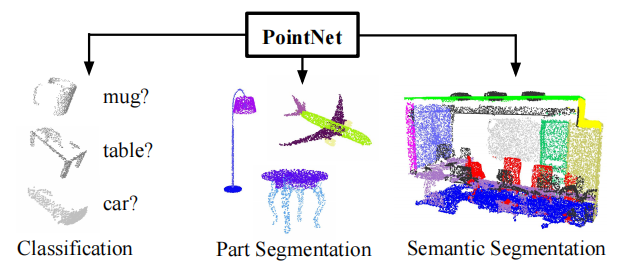
\includegraphics[scale=0.55]{doc/img/f1.png}
\end{figure}

\end{frame}

\begin{frame}
 \frametitle{问题描述}

 研究者设计了一个深度学习框架,直接使用无序点集作为输入。点云表示为一组3D点 $\{P_i | i = 1, ... ,n \} $ ,其中每个点 $P_i$ 是其 $(x,y,z)$ 坐标加上诸如颜色、法线等的额外特征通道的向量。

对于对象分类任务,Pointnet为所有 $k$ 个候选类输出 $k$ 个分数。对于语义分割,输入可以是用于部分区域分割的单个对象,或者是用于对象区域分割的3D场景。Pointnet将为 $n$ 个点中的每个点生成 $m$ 个语义类别分数,共输出 $n \times m$ 个分数。

\end{frame}

\begin{frame}
\frametitle{相关工作}

\textbf{3D计算机视觉}

Volumetric CNNs:将三维卷积神经网络应用于体素化3D视觉学习。然而,由于3D数据的稀疏性和三维卷积的计算成本,体素表示受到其分辨率的限制。FPNN和Vote3D提出了处理稀疏性问题的特殊方法,然而,处理非常大的点云仍然是一个挑战。
Multiview CNNs:将三维点云渲染成二维图像,然后应用二维卷积网络对其进行分类。通过设计良好的图像学习网络,这种方法在形状分类和检索任务上取得了主要的性能。然而,将它们扩展到场景分割或其他3D任务,如点云补全是非常困难的。
Feature-based DNNs:将三维数据转换为一个向量,然后利用全连接网络对形状进行分类。这样提取到特征的表示能力有很大的约束,因为将无序的点云转化成了有序的向量。
    
\end{frame}

\begin{frame}
\frametitle{点云特性}
无序性,与图像中的像素阵列或体素网格中的体素阵列不同,点云是一组没有特定顺序的点,输入为N个点的网络需要对N!保持输出不变性。
交互性,点云中的这些点来自于具有相同距离度量的欧几里得空间。这意味着点与点之间不是孤立的,相邻的点形成了一个相互关联的子集,这意味着模型需要从附近的点捕获局部结构的语义特征。
仿射性,点云是一个完整的仿射对象,即对整个点云进行仿射变换如旋转和平移后仍和原始点云语义特征保持一致。
    
\end{frame}
\section{PointNet}

\begin{frame}
 \frametitle{针对无序输入的对称函数}

应用点对称函数来近似点集上的一般函数,通过多层感知器网络近似 $h$ ,通过单变量函数和最大池函数的组合近似 $g$



\begin{equation*} f(\{x_{1},\ \ldots,\ x_{n}\})\approx g(h(x_{1}),\ \ldots,\ h(x_{n}))\end{equation*}



\begin{equation*} \forall\epsilon >0,\exists h,\gamma,\quad st. \left\vert f(S)-\gamma\left(\underset{x_{i}\in S}{MAX} \{h(x_{i})\}\right)\right\vert < \epsilon \end{equation*}

    
\end{frame}

\begin{frame}
\frametitle{局部特征和全局特征的聚合}

在计算全局点云特征向量之后,通过将全局特征与每个点特征拼接起来反馈给每个点。然后我们基于拼接的点特征提取新的逐点特征,其中包含了局部信息和全局信息。
    
\end{frame}

\begin{frame}
\frametitle{仿射变换对齐网络}

通过一个T-net预测仿射变换矩阵,并直接将此变换应用于输入点云,其中T-net只由简单的全连接层组成。这一思想也可以进一步扩展到特征空间的对齐。我们可以对逐点特征应用另一个对齐网络,使用同样的方法预测特征仿射变换矩阵,以对齐来自不同输入点云的特征。为了将特征变换矩阵约束为接近正交矩阵,将正则化项添加到训练损失中。

\begin{equation*} L_{reg}=\Vert I-AA^{T}\Vert_{F}^{2},\tag{2} \end{equation*}

    
\end{frame}

\begin{frame}
\frametitle{局限性}
PointNet只能捕捉点云的全局特征,不能捕获欧氏空间点集的局部结构特征,从而限制了其识别细粒度模式的能力和对复杂场景的泛化能力。
\end{frame}


\section{PointNet++}


\begin{frame}
\frametitle{分层点云特征学习}
    
使用分层特征学习代替PointNet中使用单个最大池化聚合点云特征。具体来说,每一个抽象层由一个采样层,一个分组层和一个学习层组成。

采样层,给定输入特征点集,使用迭代最远点采样(FPS)来选择特征点集的子集,与随机采样相比,在相同的质心数下,该方法对整个点集的覆盖率更高。

分组层,使用球查询搜索到质心点的特征距离在半径内的所有点(在实现中设置上限K),与kNN相比,球查询的局部邻域保证了固定的区域尺度,从而使局部区域特征在空间上更具泛化性,且利于学习层中的PointNet提取特征。

学习层,使用PointNet学习逐点特征,局部区域中的点的坐标首先被转换成相对于质心点的局部坐标系,通过PointNet得到该局部区域的全局特征作为下一个采样层的输入。




\end{frame}


\begin{frame}
\frametitle{分层点云特征学习}

\begin{figure}
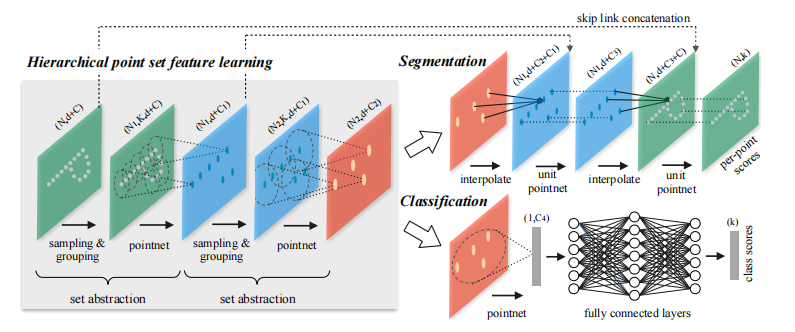
\includegraphics[scale=0.7]{doc/img/f2.png}
\end{figure}
    
\end{frame}


\begin{frame}
\frametitle{采样优化策略:非均匀采样}

多尺度分组(MSG),如图(a)所示,在每一个抽象层中使用具有不同尺度的分组层,然后根据PointNets提取每个尺度的特征。不同尺度的特征被连接以形成多尺度特征。

\begin{figure}
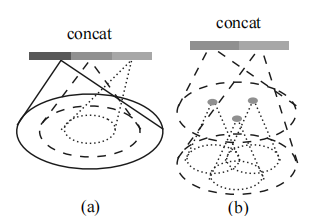
\includegraphics[scale=0.8]{doc/img/f3.png}
\end{figure}



\end{frame}

\begin{frame}
\frametitle{采样优化策略:非均匀采样}

多分辨率分组(MRG),由于上面的MSG计算开销较大,因为它在每个质心点的大规模邻域中运行PointNet。通常由于在底层时质心点的数量相当大,因此时间成本是高昂的。MRG的层特征是两个向量的拼接。一个向量(图中左侧)是通过使用单尺度分组(SSG)汇总每个子区域的特征而获得的。另一个矢量(右)是通过使用单个PointNet直接处理局部区域中的所有原始点获得的特征。当局部区域的密度低时,左侧向量比右侧向量更不可靠,因为在计算左侧向量时子区域点云稀疏导致采样不足。在这种情况下,右侧向量的权重应该更高。相反,当局部区域的密度高时,左侧矢量提供了更精细的信息,此时应该提高左侧向量的权重。


\begin{figure}
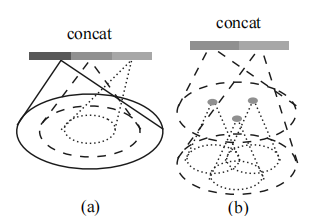
\includegraphics[scale=0.6]{doc/img/f3.png}
\end{figure}
    
    
\end{frame}


\begin{frame}
\frametitle{基于点特征传播的点云分割方法}
    
使用基于特征距离的插值传播方法逆向生成前一个抽象层所有点的近邻特征,再与前一个抽象层的分组学习特征拼接为逐点分割特征,使用PointNet的部分仿射架构进行特征学习,进行下一轮特征传播,直到传播至原始点云。在插值中,使用k个最近邻的反距离加权平均特征。


$$
f^{(j)}(x)=\frac{\sum_{i=1}^{k} w_{i}(x) f_{i}^{(j)}}{\sum_{i=1}^{k} w_{i}(x)} \quad \text { where } \quad w_{i}(x)=\frac{1}{d\left(x, x_{i}\right)^{p}}, j=1, \dots, C
$$


\end{frame}

\section{实验复现}

\begin{frame}
  \frametitle{实验环境与参数设置}

\textbf{实验环境:}

RTX 3090,Pytorch 1.10.1,Python 3.7


\textbf{参数设置:}

分类任务:batchsize为24,epoch为200,学习率为0.001,optimizer为Adam

零件分割任务:batchsize为16,epoch为251,学习率为0.001,optimizer为Adam

语义分割任务:batchsize为16,epoch为32,学习率为0.001,optimizer为Adam


\end{frame}


\begin{frame}
  \frametitle{实验数据集介绍}

\textbf{ModelNet40(用于分类任务):}

包含了40个类别(如飞机,汽车等)的CAD模型数据。训练集有9843个点云数据,测试集有2468个点云数据。

\textbf{ShapeNet(用于部件分割任务):}

包含14个大类别(如飞机,椅子等)和55个小类别的CAD模型数据。训练集有14007个点云数据,测试集有2874个点云数据。

\textbf{S3DIS(用于语义分割任务):}

是大规模室内三维空间数据集,包含了6个建筑物,共计271个房间。房间内包含13类物体(如天花板、地板、门、沙发等) 。



\end{frame}


\begin{frame}
  \frametitle{数据集可视化}
\textbf{ModelNet40(分类任务):}

源数据(txt文件)进行可视化:


\begin{figure}
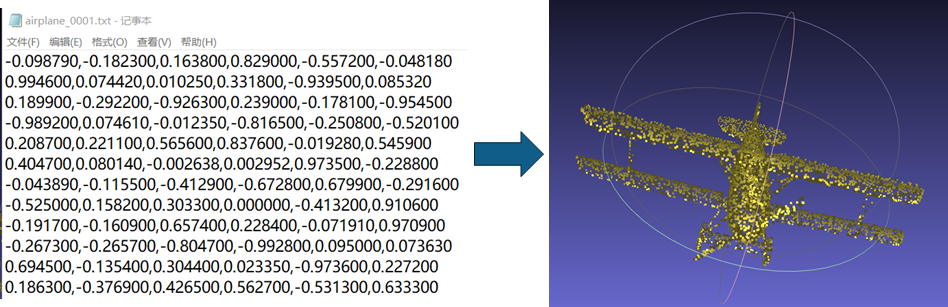
\includegraphics[scale=0.4]{doc/img/f4.png}
\end{figure}



\end{frame}



\begin{frame}
  \frametitle{数据集可视化}

\textbf{ShapeNet(部件分割任务)}

源数据(txt文件)进行可视化:


\begin{figure}
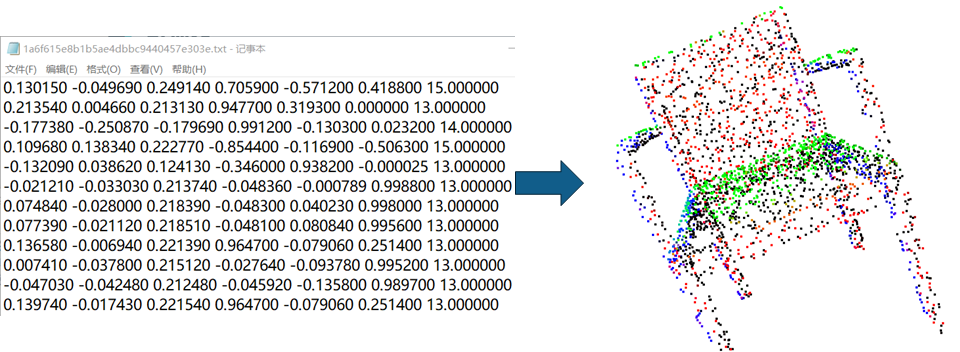
\includegraphics[scale=0.35]{doc/img/f5.png}
\end{figure}


\end{frame}


\begin{frame}
  \frametitle{数据集可视化}

\textbf{S3DIS(语义分割任务)}

源数据(txt文件)进行可视化:


\begin{figure}
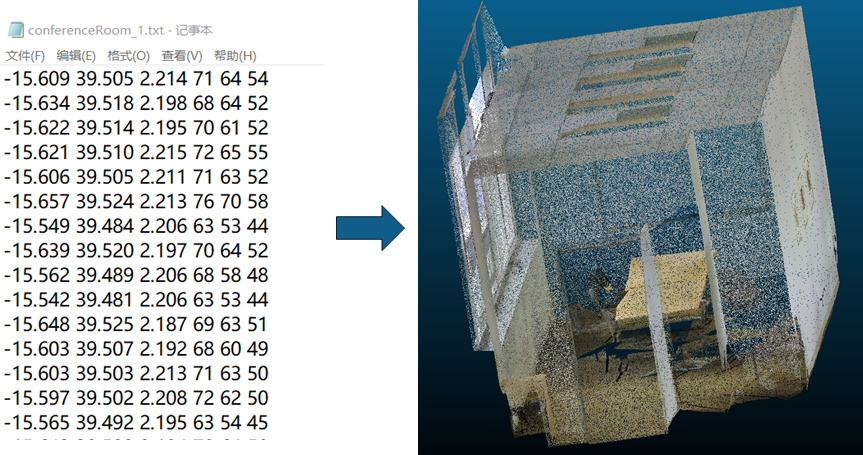
\includegraphics[scale=0.3]{doc/img/f6.png}
\end{figure}


\end{frame}


\begin{frame}
  \frametitle{实验复现结果及分析}

在ModelNet40数据集上进行分类:

\begin{figure}
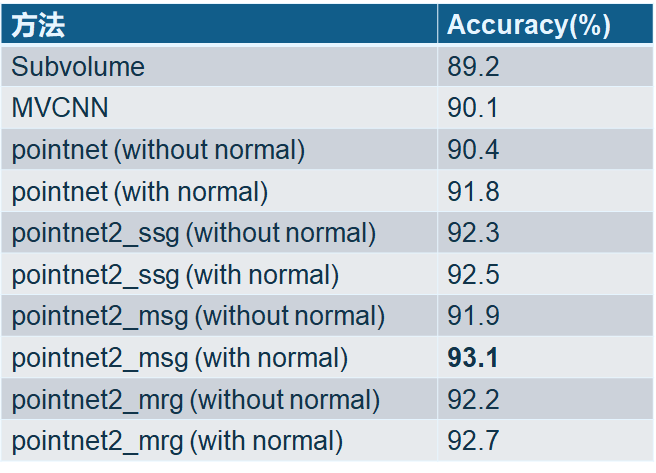
\includegraphics[scale=0.35]{doc/img/t1.png}
\end{figure}


% \begin{table}[h]
%   \centering
%   % \caption{}
%   \label{tab:q}
%   \begin{tabular}{ccccc}
%     \toprule
% 方法          & Accuracy( \% )\\
%     \midrule
% Subvolume         & 89.2 \\ \hline
% MVCNN           & 90.1 \\ \hline
% pointnet (without normal) & 90.4 \\ \hline
% pointnet (with normal) & 91.8 \\ \hline
% pointnet2\_ssg (without normal) & 92.3 \\ \hline
% pointnet2\_ssg (with normal) & 92.5 \\ \hline
% pointnet2\_msg (without normal) & 91.9 \\ \hline
% pointnet2\_msg (with normal) & 93.1 \\ \hline
% pointnet2\_mrg (without normal) & 92.2 \\ \hline
% pointnet2\_mrg (with normal) & 92.7 \\ \hline
%     \bottomrule
%   \end{tabular}
% \end{table}

\end{frame}


\begin{frame}
  \frametitle{实验复现结果及分析}

比较pointnet和pointnet++各个模型的显存占用:

\begin{figure}
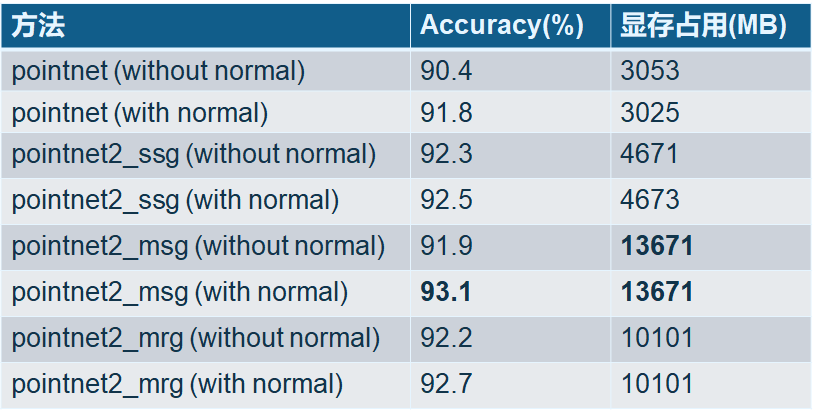
\includegraphics[scale=0.35]{doc/img/t2.png}
\end{figure}



\end{frame}



\begin{frame}
  \frametitle{实验复现结果及分析}

在ShapeNet数据集上进行部件分割:

\begin{figure}
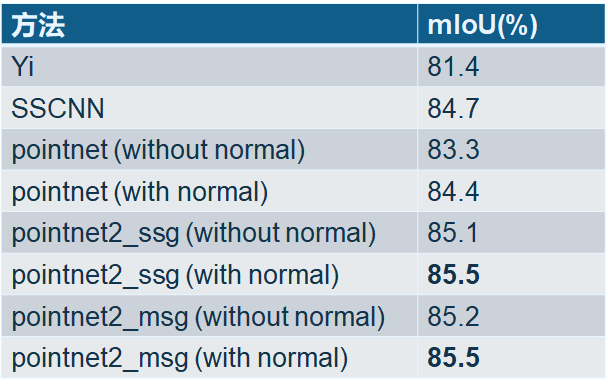
\includegraphics[scale=0.35]{doc/img/t3.png}
\end{figure}


\end{frame}

\begin{frame}
  \frametitle{实验复现结果及分析}

在S3DIS数据集上进行语义分割:


\begin{figure}
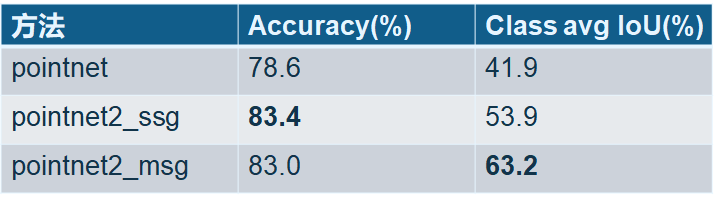
\includegraphics[scale=0.35]{doc/img/t4.png}
\end{figure}

\end{frame}


\begin{frame}
  \frametitle{S3DIS语义分割结果可视化}

\begin{figure}
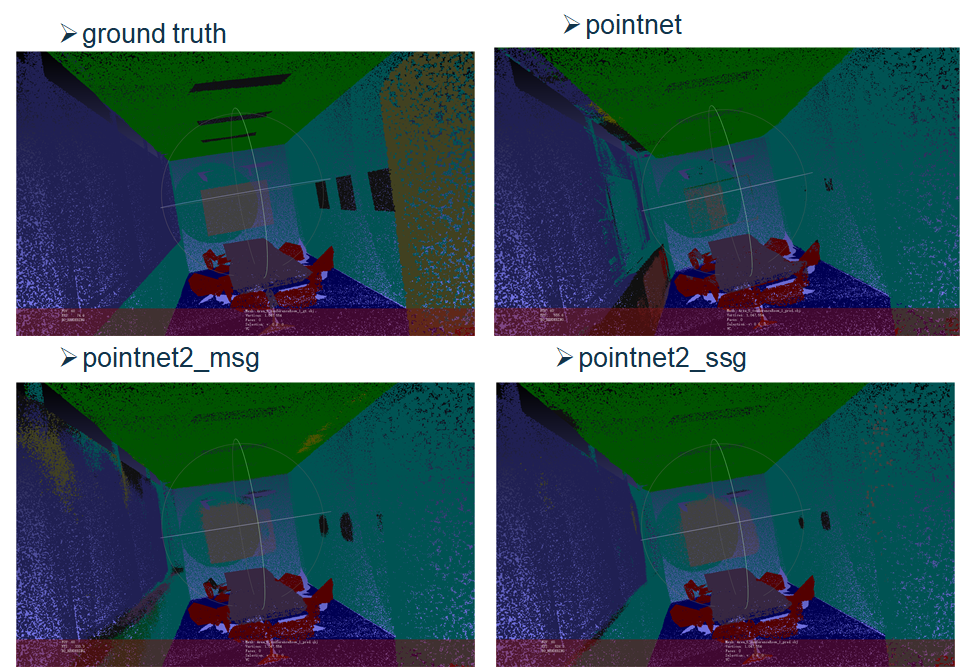
\includegraphics[scale=0.3]{doc/img/f7.png}
\end{figure}


\end{frame}


\section{MRG方法实现}

\begin{frame}{MSG与MRG}
    \begin{columns}
        \begin{column}{0.50\textwidth}
            \begin{block}{MSG}
                \begin{itemize}
                    \item 为了提取多尺度的模式,一种简单有效的方法是对于每层的点云都采用多个尺寸的局部区域进行特征聚合
                \end{itemize}
            \end{block}
            \begin{block}{MRG}
                \begin{itemize}
                    \item MSG方法计算成本较高,替代方法MRG通过连接不同层特征,在减少计算成本的同时仍保留多尺度模式提取能力
                \end{itemize}
            \end{block}
        \end{column}
        \begin{column}{0.50\textwidth}
            \begin{figure}
                \centering
                \includegraphics[width=0.6\textwidth]{doc/img/MRG与MSG.png}
                \caption{MSG与MRG}
                \label{fig:MSG-MRG}
            \end{figure}
        \end{column}
    \end{columns}
\end{frame}

\begin{frame}{使用MRG的分类网络结构}
    \begin{columns}
        \begin{column}{0.50\textwidth}
            \begin{block}{}
                \begin{itemize}
                    \item 论文并没有给出MRG方法的源码,我们根据论文中给出的网络结构实现了使用MRG的分类pointnet++
                    \item 右图是论文中的pointnet++的网络结构
                \end{itemize}
            \end{block}
        \end{column}
        \begin{column}{0.50\textwidth}
            \begin{figure}
                \centering
                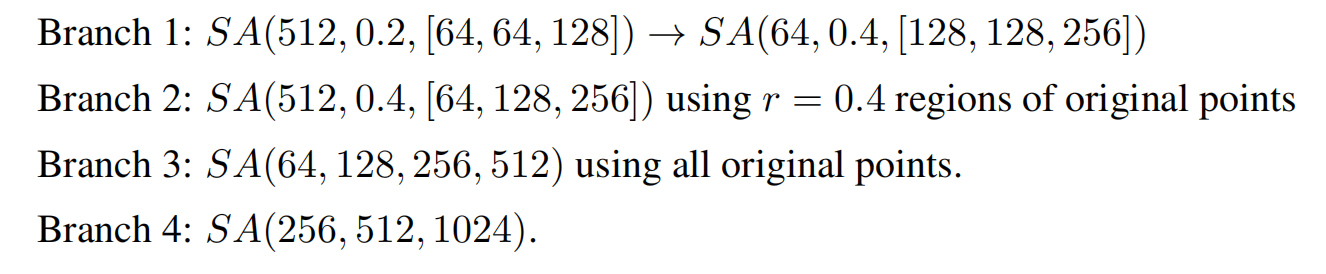
\includegraphics[width=0.9\textwidth]{doc/img/论文网络结构.png}
                \caption{MRG分类网络结构}
                \label{fig:structure}
            \end{figure}
        \end{column}
    \end{columns}
\end{frame}
\begin{frame}{使用MRG的分类网络结构}
    \begin{columns}
        \begin{column}{1\textwidth}
            \begin{block}{}
                \begin{itemize}
                    \item SA为Set Abstraction;(N,D)表示输入点数为N,特征维度为D;C表示连接操作
                \end{itemize}
            \end{block}
            \begin{figure}
                \centering
                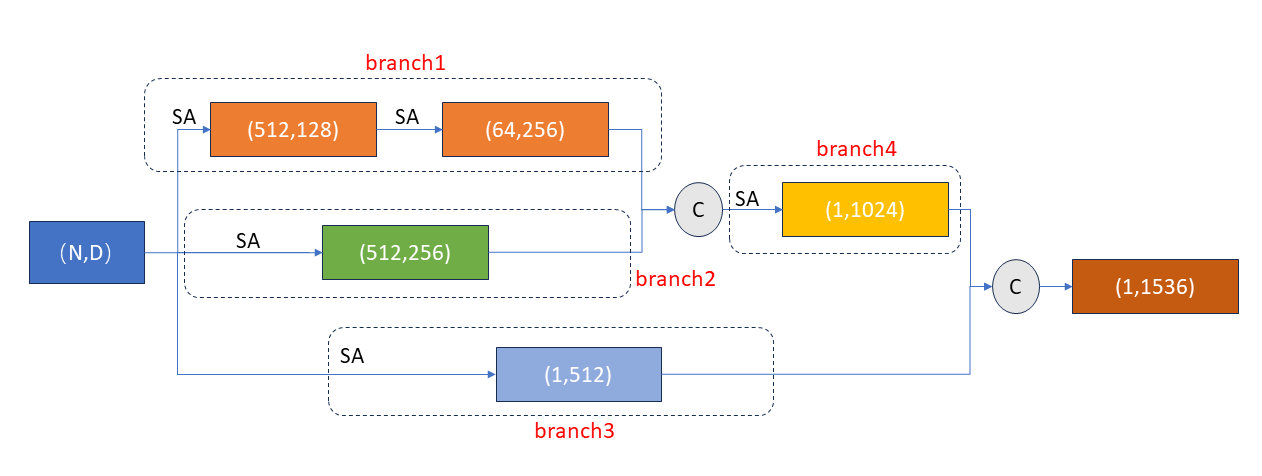
\includegraphics[width=0.8\textwidth]{doc/img/网络示意图.png}
                \caption{特征提取过程示意图}
                \label{fig:network}
            \end{figure}
        \end{column}
    \end{columns}
\end{frame}








\begin{frame}
  \frametitle{致谢}
  \centerline{\Large 谢谢!}
\end{frame}

\end{document}
